\begin{defn} 
We say that \(\Sigma\) is \emph{area minimizing} if every compact piece of \(\Sigma\) with smooth boundary minimizes the \(n\)-area among all other hypersurfaces with same boundary. In other words, \(\Sigma\) is area minimizing if for each compact set \(K \subset \R^{n+1}\) such that \(\Sigma \cap K\) is a smooth compact hypersurface with smooth boundary, then for every other compact hypersurface \(\Sigma'\) with \(\de \Sigma' = \de(\Sigma \cap K)\) we have
\[
    \Haus^n(\Sigma \cap K) \le \Haus^n(\Sigma')
\]
\end{defn}

A sufficient condition for being area minimizing is being \emph{calibrated}. 
\begin{defn}
    A calibration for \(\Sigma\) is a smooth vector field \(v \colon \R^{n+1} \to \R^{n+1}\) such that
    \begin{itemize}
        \item \(|v|\le 1\) on \(\R^{n+1}\);
        \item \(v \cdot \nu =1 \) on \(\Sigma\);
        \item \(\dive v = 0\) on \(\R^{n+1}\).
    \end{itemize}
\end{defn}
In particular, for every compact hypersurface \(\Sigma'\) (which necessarily is two-sided)
\[
    \int_{\Sigma'} v \cdot \nu' \dif \Haus^n \le \Haus^n(\Sigma')
\]
for any unit normal vector field \(\nu' \colon \Sigma' \to \Sp^n\).
\begin{lemma}
    If \(\Sigma\) is calibrated then it's area minimizing.
\end{lemma}
\begin{proof}
    Let \(\de \Sigma' = \de(\Sigma \cap K)\). Since transversality is an open condition, we can assume that \(\Sigma'\) meets \(\Sigma\) transversely. Moreover, up to consider each piece individually, we may also assume that \(\Sigma'\) is on one side of \(\Sigma\). In this case, we can find an open domain \(\Omega \subset \subset \R^{n+1}\) such that \(\de\Omega= \Sigma' \cup (\Sigma \cap K)\). Then by the divergence theorem
    \[
        \Haus^n(\Sigma') -\Haus^n(\Sigma\cap K) \ge \int_{\Sigma'} v \cdot \nu' \dif \Haus^n - \int_{\Sigma \cap K} v \cdot \nu \dif \Haus^n  = \pm \int_\Omega \dive v \dif x= 0,
    \]
    as required.
\end{proof}

An entire minimal graph is always calibrated by
\[
    v = \frac{(-\nabla u,1)}{\sqrt{1+|\nabla u|^2}},
\]
so in particular it's area minimizing. 

We are going to use three important features of area minimizing hypersurfaces:
\begin{itemize}
    \item stability
    \item extrinsic volume growth estimate
    \item weak* closure.
\end{itemize}

\subsection{Stability}
\begin{defn}
    A minimal hypersurface is \emph{stable} if for every \(\vp \in C^\infty_c(\Sigma)\), letting \(\Sigma_t \coloneq \{ x+t\vp(x)\nu(x) \colon x \in \Sigma\}\),
    \[
        \left.\frac{\dif^2}{\dif t^2}\right|_{t=0} \Haus^n(\Sigma_t) \ge 0.
    \]
\end{defn}
\begin{thm}[Second variation formula]
    Let \(\Sigma \subset \R^n\) be a minimal hypersurface. For every \(\vp \in C^\infty_c(\Sigma)\), let \(\Sigma_t \coloneq \{ x+t\vp(x)\nu(x) \colon x \in \Sigma\}\). 
    Then
    \begin{equation}
        \left.\frac{\dif^2}{\dif t^2}\right|_{t=0}\Haus^n(\Sigma_t) = \int_\Sigma |\nabla_\Sigma\vp|^2-|A_\Sigma|^2\vp^2 \dif \Haus^n = - \int_\Sigma \vp L_\Sigma \vp \ \dif \Haus^n,
    \end{equation}
    where
    \[
        L_\Sigma = \Delta_\Sigma + |A_\Sigma|^2
    \]
    is the \emph{Jacobi operator} of \(\Sigma\).
\end{thm}

Therefore a minimal hypersurface \(\Sigma \subset \R^{n+1}\) is stable if and only if the \emph{stability inequality} holds
\begin{equation}\label{eq: stability inequality}
    \int_\Sigma |\nabla_\Sigma \vp|^2 - |A_\Sigma|^2\vp^2\dif \Haus^n \ge 0 \qquad \forall \vp \in C^\infty_c(\Sigma).
\end{equation}
Observe that, in particular, every area minimizing hypersurface is stable.

Since \(L_\Sigma\) is self-adjoint elliptic operator, setting homogeneous boundary conditions it can be diagonalized on every relatively compact domain \(\Omega \subset \subset \Sigma\), and the first eigenvalue can be characterized as
\[
    \lambda_1(\Omega) \coloneq \inf \left\{ \frac{\int_\Omega |\nabla_\Sigma \vp|^2 - |A_\Sigma|^2 \vp^2 \dif \Haus^n}{\int_\Omega \vp^2 \dif \Haus^n} \colon \vp \in C^\infty_c(\Omega) \setminus\{0\} \right\}.
\]
Therefore, \(\Sigma\) is stable if and only if
\[
    d_0(\Sigma) \coloneq \inf_{\Omega \subset \subset \Sigma} \lambda_1(\Omega) \ge 0.
\]

\subsection{Extrinsic volume growth estimate}
\begin{thm}\label{thm: quadratic area growth for entire minimal graphs}
	If \(\Sigma\) is a complete area minimizing hypersurface in \(\R^{n+1}\), then for all \(r>0\)
	\[
		\Haus^n(\gr(u) \cap B_r) \leq \frac{(n+1)\omega_{n+1}}{2} r^n
	\]
	where \(B_r=B_r(0)\) is the ball of \(\R^{n+1}\) centered at the origin with radius \(r\) and \((n+1)\omega_{n+1}\) is the \(\Haus^n\)-measure of the standard unit sphere \(\Sp^n \subset \R^{n+1}\).
\end{thm}
 
\begin{proof}
	By Sard's theorem the set of positive real numbers \(r>0\) such that \(\Sigma\) intersects \(S_r\coloneq \de B_r\) transversely is dense in \(\R_{>0}\), so we can prove the statement assuming that \(\Sigma\) intersects \(S_r\) transversely. Assume also that \(\Gamma \coloneq \Sigma \cap S_r \ne \varnothing\). The implicit function theorem implies that \(\Gamma\) is a (compact, but possibly non connected) \((n-1)\)-dimensional manifold without boundary. By Jordan-Brouwer separation theorem, each connected component \(\Gamma_j\) of \(\Gamma\) separates \(S_r\) into two connected components having boundary \(\Gamma_j\), and in this way we can write \(S_r \setminus \Gamma= \Sigma_1 \sqcup \Sigma_2\) with \(\Sigma_1, \Sigma_2\) having common boundary \(\Gamma\) (see Figure~\ref{fig: connected components}). 
    \begin{figure}[ht] 
		\centering
		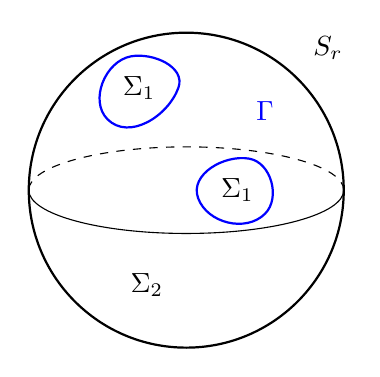
\begin{tikzpicture}
		%\draw[help lines] (-3,-3) grid (3,3);
		\draw [thick] (0,0) circle (2);
		\draw (-2,0) arc (180:360: 2 and 0.55);
		\draw [dashed] (2,0) arc (0:180: 2 and 0.55);
		
		\draw[thick, blue] (-1,.9) to[out=-45, in= 250] (-.1,1.3) to[out=70,in=10] (-.7,1.7) to [out=190, in=135](-1,.9);
		\draw[thick, blue] (1,-.3) to[out=-135, in= 290] (.15,-.1) to[out=110,in=170] (.8,.4) to [out=350, in=45](1,-.3);
		
		\node at (1.8,1.8) {\(S_r\)};
		\node at (-.6,1.3) {\(\Sigma_1\)};
		\node at (.65,0) {\(\Sigma_1\)};
		\node at (-.5,-1.2) {\(\Sigma_2\)};
		\node[blue] at (1,1) {\(\Gamma\)};
		\end{tikzpicture}
        \caption{Construction of the competitors \(\Sigma_1\) and \(\Sigma_2\).}
        \label{fig: connected components}
	\end{figure}
    Moreover,
    \[
		(n+1)\omega_{n+1}r^n = \Haus^n(S_r) = \Haus^n(\Sigma_1) + \Haus^n(\Sigma_2).
	\]
	Since \(\Sigma\) is area minimizing and \(\de (\Sigma \cap B_r)=\Gamma=\de \Sigma_1=\de \Sigma_2\), we deduce that
	
	\[
	2 \Haus^n( \Sigma \cap B_r (0)) \leq \Haus^n(\Sigma_1) + \Haus^n(\Sigma_2) = (n+1)\omega_{n+1}r^{n}. \qedhere
	\]
\end{proof}

\subsection{Closure of area minimizing currents}

\begin{defn}
    An \emph{integer rectifiable \(k\)-current} \(T\) is an element of the topological dual of the space of smooth compactly supported \(k\)-forms of \(\R^{n+1}\) which admits a representation
    \[
        \langle T , \omega \rangle = \sum_{j=1}^\infty \theta_j \int_{K_j} \omega 
    \]
    where \(\theta_j \in \Z\) and \(K_j \subset \Sigma_j\) are closed subsets of oriented \(k\)-dimensional \(C^1\)-submanifolds \(\Sigma_j\) of \(\R^{n+1}\). The class of integral \(k\)-currents in \(\R^{n+1}\) is denoted by \(\mathcal{I}_k(\R^{n+1})\). 
    
    The \emph{support} of a current \(T \in \mathcal{D}_k(\R^{n+1})\) is the complement of the maximal open set \(A\) such that \(\langle T,\omega \rangle = 0\) for every \(\omega \in \mathcal{D}^k(\R^{n+1})\) with \(\spt(\omega) \subset A\). The \emph{mass measure} of \(T\) is defined by
    \[
    \begin{aligned}
        \|T\|(\Omega) &\coloneq \sup \left\{ \langle T,\omega \rangle \colon \omega \in \mathcal{D}^k(\R^{n+1}), \|\omega\|_\infty \le 1\right\}  &&\text{if }\Omega \subset \R^{n+1} \text{ open}, \\
        \|T\|(E) &\coloneq \inf\{ \mu_T(\Omega) \colon \Omega \supset E \text{ open}\}  &&\text{if }E\subset \R^{n+1} \text{ Borel}.
    \end{aligned}
    \]
    The \emph{boundary} of \(T\) is the \((k-1)\)-current \(\de T \in \mathcal{D}_{k-1}(\R^{n+1})\) defined by forcing Stokes' theorem:
    \[
        \langle \de T, \vp \rangle \coloneq \langle T , \dif \vp \rangle \qquad \forall \vp \in \mathcal{D}_{k-1}(\R^{n+1}).
    \]
\end{defn}

The integer rectifiable current generated by a \(C^1\)-submanifold \(\Sigma\) is denoted by \(\llbracket \Sigma \rrbracket\).

Integer rectifiable currents are endowed with the weak* topology of Radon measures, i.e., if \(T_j, T \in \mathcal{I}_k(\R^{n+1})\), we say that \(T_j \weakstarto T\) if 
\[
    \langle T_j, \omega \rangle \to \langle T,\omega \rangle \qquad \forall\omega \in \mathcal{D}^k(\R^{n+1}).
\]

It holds the following compactness result (cf \cite[Chapter~6]{Simon_GMT1983})
\begin{thm}[Compactness, Federer-Fleming]
    If \((T_j)_j \subset \mathcal{I}_k(\R^{n+1})\) is such that for every \(\Omega \subset \subset \R^{n+1}\)
    \[
        \sup_j \mu_{T_j}(\Omega) + \mu_{\de T_j}(\Omega) < \infty,
    \]
    then \(T_j\) admits a weak* converging subsequence in \(\mathcal{I}_k(\R^{n+1})\).
\end{thm}

\begin{defn}
    An integral current \(T \in \mathcal{I}_n(\R^{n+1})\) is \emph{area minimizing} if for every \(\Omega \subset \subset \R^{n+1}\) and \(S \in \mathcal{I}_n(\R^{n+1})\) such that \(\de S=\de T\) and \(\spt(T-S) \subset \Omega\),
    \[
        \mu_T(\Omega) \le \mu_S(\Omega).
    \]
\end{defn}

Clearly, if \(\Sigma\) is an area minimizing hypersurface, the corresponding current \(\llbracket \Sigma \rrbracket\) is area minimizing as well.

Since \(T_j \weakstarto T\) implies that \(\de T_j \weakstarto \de T\) and \(\|T_j\| \weakstarto \|T\|\), the lower semicontinuity on open sets implies the following.
\begin{prop}[Closure of area minimizing currents]\label{prop: closure of area minimizing currents}
    If \(T_j \weakstarto T\) in \(\mathcal{I}_n(\R^{n+1})\) and each \(T_j\) is area minimizing with same boundary, then \(T\) is also area minimizing.
\end{prop}

\begin{defn}
    Let \(\phi \colon \R^{n+1} \to \R^{n+1}\) be a \(C^1\)-diffeomorphism and \(T \in \mathcal{I}_k(\R^{n+1})\). The \emph{push-forward}  of \(T\) along \(\phi\) is the integral current \(\phi_\#T\) defined by
    \[
        \langle \phi_\#T, \omega \rangle = \langle T, \phi^*\omega \rangle \qquad \forall \omega \in \mathcal{D}^k(\R^{n+1}).
    \]

    A current \(T \in \mathcal{I}_n(\R^{n+1})\) is \emph{stationary} if for every smooth 1-parameter family of diffeomorphisms \(\phi \colon \R^{n+1} \times (-\eps,\eps) \to \R^{n+1}\) with \(\phi_0 = \id\) and \(\phi|_{\R^{n+1}\setminus \Omega} = \phi_t|_{\R^{n+1}\setminus \Omega}\) for every \(t\) and some \(\Omega\subset \subset \R^{n+1}\) with \(\spt(\de T) \subset \R^{n+1}\setminus \Omega\),
    \[
        \left. \frac{\dif }{\dif t}\right|_{t=0} \|(\phi_t)_\#T\|(\Omega) = 0.
    \]
\end{defn}

\begin{rmk}
    An area-minimizing current is stationary.
\end{rmk}

\begin{defn}
    Given an integer rectifiable current \(T \in \mathcal{I}_n(\R^{n+1})\), a point \(x \in \spt(T)\) is a regular point of \(T\) if there exists \(r>0\) such that \(\spt(T) \cap B_r(x)\) is a smooth hypersurface of \(\R^{n+1}\). The set of regular points of \(T\) is denoted by \(\Reg(T)\) and \(\Sing(T) \coloneq \spt(T)\setminus \Reg(T)\) is the set of singular points of \(T\). The \emph{regularity scale} of \(T\) is the function \(r_T \colon \spt(T) \to [0,+\infty]\) defined as \(r_T(x)=0\) if \(x \in \Sing(T)\) and 
    \[
        r_T(x) \coloneq \sup \left\{ r>0 \colon \spt(T)\cap B_r(x) \text{ smooth hypersurface with }|A|^2\le r^{-1} \right\}
    \]
    if \(x \in \Reg(T)\). The set also
    \[
        \mathcal{R}_{\ge \rho} (T) \coloneq \{ x \in \spt(T) \colon r_T(x) \ge \rho\}
    \]
    for every \(\rho>0\).
\end{defn}

\subsection{The monotonicity formula}

\begin{thm}[Monotonicity formula]\label{thm: monotonicity formula}
    Let \(T\) be an area minimizing integer rectifiable \(n\)-current in \(\R^{n+1}\) with \(\de T=0\). Then for all \(0<s<r < \infty\),
    \begin{equation*}
        \frac{\|T\|(B_r(p))}{r^n} - \frac{\|T\|(B_s(p))}{s^n} = \int_{A(p,s,r)} \frac{|\nabla^\perp (x-p)|^2}{|x-p|^{n}} \ \dif \|T\|(x),
    \end{equation*}
    where \(A(p,s,r) = B(p,r) \setminus \overline{B(p,s)}\).

    In particular, denoting by \(\omega_n\) the Lebesgue measure of the Euclidean unit ball of \(\R^n\), the \emph{density function}
    \[
        \Theta_T(p,r) \coloneq \frac{\|T\|(B(p,r))}{\omega_n r^n}
    \]
    is non decreasing and it's constant if and only if \(T\) is a cone with vertex \(p\), i.e., \((\eta_{p,\lambda})_\# T = (\eta_{p,0})_\#T\) for every \(\lambda>0\).
\end{thm}

The monotonicity formula does not depend on the orientation, and in fact it extends in the larger class of \emph{stationary varifolds}. The idea of the proof is to test the radial vector field \(X(x)=x-p\) in the first variation formula. For the details see \cite[Chapter~8,\S3]{Simon_GMT1983}.